\section{Basics of digital image filtering}\label{sec:basic-img-filtering}

\subsection{Linear Filtering}\label{sec:bif-linear}

\textit{Image filtering} is the process of applying some function to local image patches. Its goals are: reduce noise, fill-in missing values, extract image features.

\textit{Linear filtering} is the simplest case of image filtering: replace each pixel by a linear combination of its neighbors.

\textit{2D discrete convolution} is an example of linear filtering and is computed as follows:
\begin{equation}\label{eq:conv2d}
    f[m,n] = I \otimes g = \sum_{k,l} I[m-k, n-l] \cdot g[k,l],
\end{equation}
that is, obtain the value of the pixel in position $(m,n)$ of the filtered image $f$ as the cross product of:
\begin{myitem}
    \item a portion of the original image $I$ given by the corresponding pixel and a number of neighbors given by the size of the kernel, i.e. $k \times l$, and
    \item the kernel $g$ itself.
\end{myitem}
The operation, repeated for all the pixels of the image, corresponds to this process:
\begin{myitem}
    \item mirror the filter across both dimensions (because of the minus sign),
    \item swipe it across the image,
    \item multiply and sum.
\end{myitem}

Analogously, if we have a 1D-filter and a 2D image, the convolution operation is:
\begin{equation}\label{eq:conv1d}
    f[m,n] = I \otimes g = \sum_{k} I[m-k, n] \cdot g[k].
\end{equation}

Examples:
\begin{myitem}
    \item with a filter $[0,0,0,0,1,0,0,0,0]$ the image stays the same, since the considered pixel is copied and the neighbors are ignored;
    \item with a filter $[0,0,0,0,0,0,0,1,0]$ the image is shifted on the left of 3 pixels, since the filter is mirrored and so the considered pixel is copied in the position of its third neighbor on the left;
    \item with a filter $[0,0,0,1,1,1,0,0,0]$ the image is blurred, since the new pixel is obtained by the average of the considered pixel and its immediate neighbors.
\end{myitem}

Note that it's usually preferable that the elements of the filter vector sum up to 1, especially in a neural network where there are many convolutional filters.

Let's recall some basic properties of linear systems:
\begin{myitem}
    \item homogeneity: $T[a \cdot X] = a \cdot T[X]$,
    \item additivity: $T[X_1 + X_2 ] = T[X_1] + T[X_2]$,
    \item superposition: $T[a \cdot X_1 + b \cdot X_2 ] = a \cdot T[X_1] + b \cdot T[X_2]$,
    \item linear systems $\Longleftrightarrow$ superposition.
\end{myitem}

Thus, since those filters are linear, they can be combined to obtain new filters:
\begin{equation}\label{eq:conv-combined}
    f[m,n] = I \otimes g_1 - I \otimes g_2 = I \otimes \left(g_1 - g_2\right).
\end{equation}
Example: with a filter $[0,0,0,0,2,0,0,0,0] - [0,0,0,1,1,1,0,0,0]$ the image is sharpened, since we enhance the considered filter before applying blur.

Furthermore, it is also true that
\begin{equation}\label{eq:conv-separable}
    f[m,n] = \left(g_1 \otimes g_2\right) \otimes I = g_1 \otimes \left(g_2 \otimes I\right),
\end{equation}
that is, the filtered image $f$ can be obtained by first applying one filter, and then another, or by applying directly their composition. If a 2D filter can be written as the product of two 1D filter (one in $x$-direction and one in $y$-direction), it's called \textbf{separable}.


\subsection{Filtering to Reduce Noise}\label{sec:bif-noise}

Filtering can be applied to reduce \textbf{noise}, such as light fluctuations, sensor noise, quantization effects, finite precision (low-level noise) or shadows, extraneous objects (complex noise). To do this, we assume that the neighborhood of a pixel contains information about its intensity.

We use the additive noise model: image $I$ = signal $S$ + noise $N$, and the intensity of the $i$-th pixel is $I_i = S_i + N_i$ with $E(N_i) = 0$, where $S_i$ is deterministic and $N_i, N_j$ are IID for $i \neq j$. Therefore, averaging noise reduces its effect and smoothing can give an inference about the original signal.\label{noise-iid}

The \textbf{average filter} replaces each pixel with an average of its neighborhood. If all weights are equal, it is called a \textbf{box} filter (and it is separable).

A smarter average filter is the \textbf{Gaussian filter}:
\begin{myitem}
    \item It's rotationally symmetric;
    \item It weights nearby pixels more than distant ones (probabilistic inference);
    \item The ``amount'' of smoothing depends on the parameter $\sigma$ of the Gaussian;
    \item It is separable (see \ref{eq:conv-separable}), thus we have the Gaussian in $x$-direction
    \begin{equation}\label{eq:gauss-x}
        g(x) = \frac{1}{\sqrt{2\pi} \cdot \sigma} \cdot e^{-\frac{x^2}{2\sigma^2}},
    \end{equation}
    the Gaussian in $y$-direction
    \begin{equation}\label{eq:gauss-y}
        g(y) = \frac{1}{\sqrt{2\pi} \cdot \sigma} \cdot e^{-\frac{y^2}{2\sigma^2}},
    \end{equation}
    and the Gaussian in both directions
    \begin{equation}\label{eq:gauss-xy}
        g(x,y) = \frac{1}{2\pi\sigma^2} \cdot e^{-\frac{x^2 + y^2}{2\sigma^2}};
    \end{equation}
    \item Let's prove the Gaussian's separability:
    \begin{flalign*}
        h(i,j) &= f(i,j) \cdot g(i,j)&\\
        &= \sum_{k=1}^{m} \sum_{l=1}^{n} g(k,l) \cdot f(i-k, j-l)&\\
        &= \sum_{k=1}^{m} \sum_{l=1}^{n} e^{-\frac{k^2 + l^2}{2\sigma^2}} \cdot f(i-k, j-l)&\\
        &= \sum_{k=1}^{m} e^{-\frac{k^2}{2\sigma^2}} \left[ \underbrace{\sum_{l=1}^{n} e^{-\frac{l^2}{2\sigma^2}} f(i-k, j-l)}_{h'} \right]&\tag{apply 1-D Gaussian horizzontally}\\
        &= \sum_{k=1}^{m} e^{-\frac{k^2}{2\sigma^2}} \cdot h'(i-k, j-l)&\tag{apply 1-D Gaussian vertically}
    \end{flalign*}
\end{myitem}

\begin{figure}[!h]
    \centering
    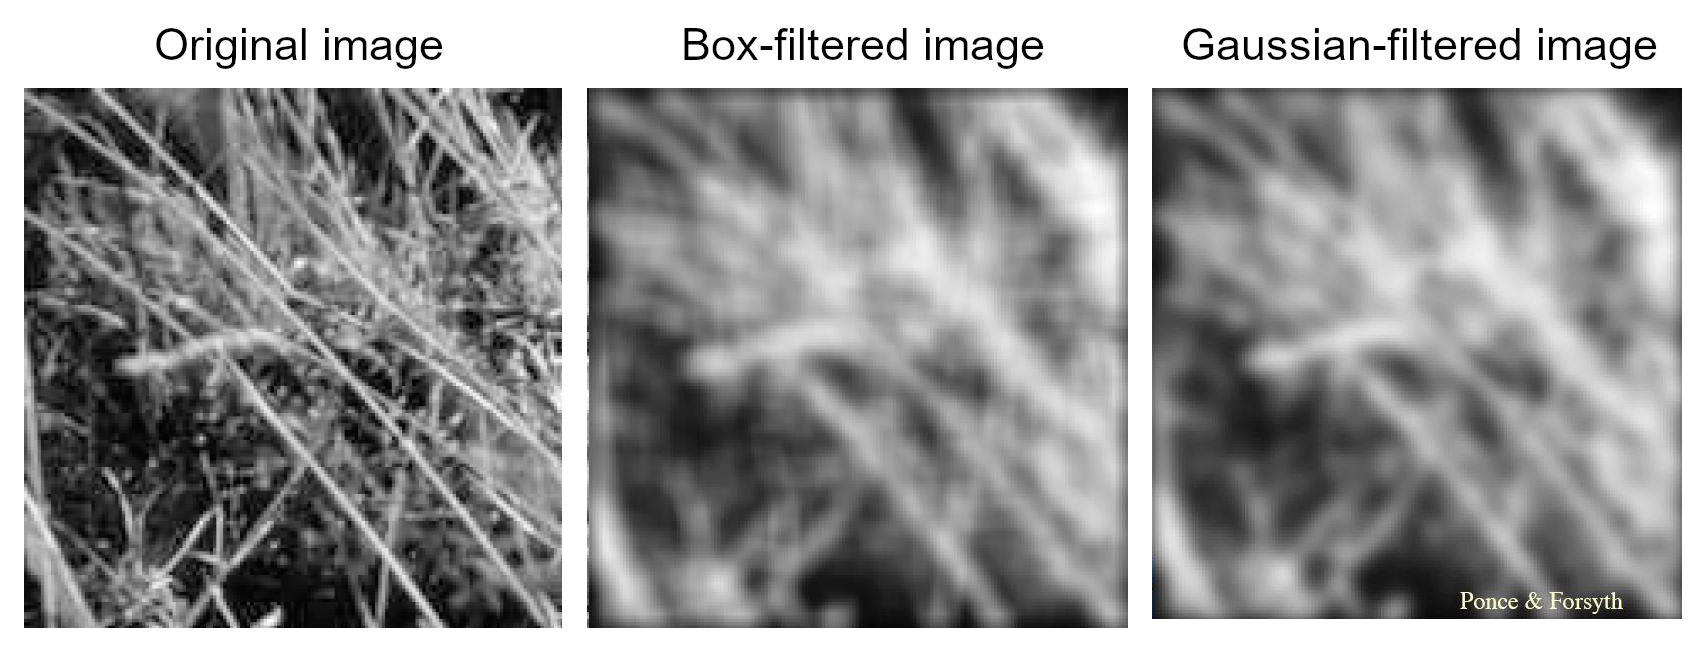
\includegraphics[width=.9\textwidth]{gaussian-filter}
    \caption[Gaussian Pyramid]{Gaussian and Box filters}
    \label{fig:gaussian-filter}
\end{figure}


\subsection{Multi Scale Image Representation}\label{sec:bif-multi-scale}

To classify objects, a possibility is to compare the image with a set of objects' templates, used as kernels. Since it is very computationally expensive to execute a convolution with a big kernel, it is preferable to store small kernels, but in this manner you can't find bigger objects.

Thus, you can build a \textbf{Gaussian Pyramid}: repeatedly blur and down-sample the image, so that you obtain smaller and smaller images, until you find an object or the image reaches the size of the template/kernel. The blurring is quite fast since you can use a small linear filter, and the down-sampling is even faster since it is sufficient to remove a certain percentage of the pixels of the image.\label{gaussian-pyramid}

\begin{figure}[!h]
    \centering
    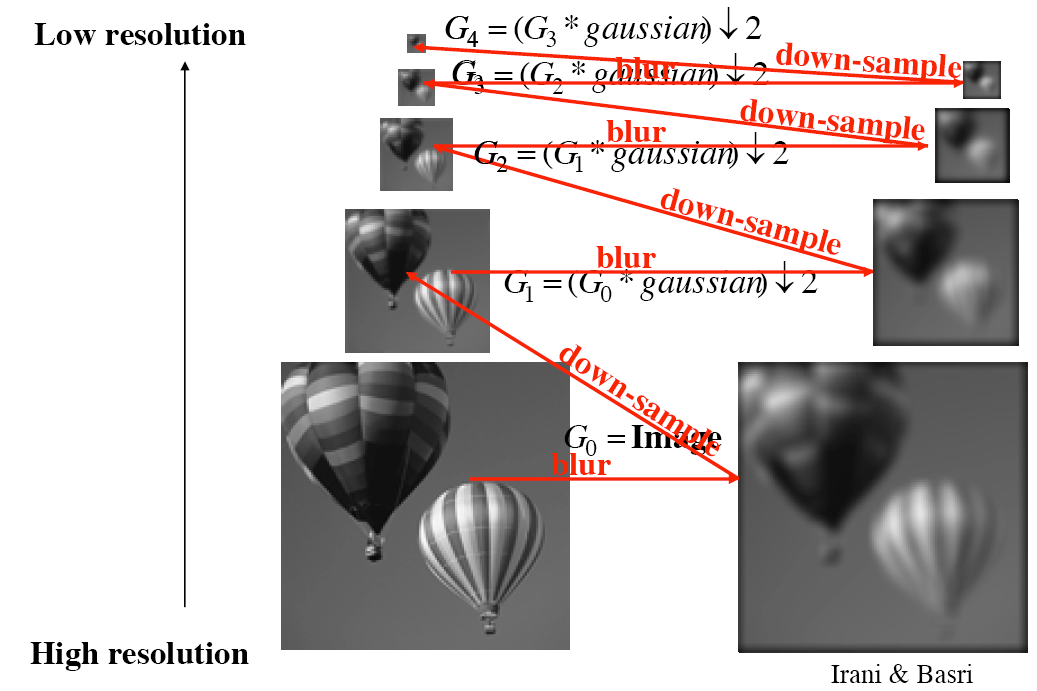
\includegraphics[width=.8\textwidth]{gaussian-pyramid}
    \caption[Gaussian Pyramid]{Gaussian Pyramid}
    \label{fig:gaussian-pyramid}
\end{figure}


In this way, you loose the details but you maintain average colors and shapes. That is, if you consider the image as made of light waves, you can apply the \textit{Fourier Transform} to decompose those waves into a sum of sinusoidal curves (the original wave is is better approximated if you continue adding waves with higher frequency).
Then, to blur and down-sample the image means to remove the waves with higher frequency.


\subsection{Edge Detection}\label{sec:bif-edge}

David Lowe's approach to recognition and localization:
\begin{myenum}
    \item Filter image to find brightness changes,
    \item Fit lines to the raw measurements,
    \item Project model into the image and match to lines (solving for 3D pose).
\end{myenum}

\begin{figure}[!h]
    \centering
    \includegraphics[width=\textwidth]{"lowe"}
    \caption[Lowe's method]{Lowe's method}
    \label{fig:lowe}
\end{figure}

The common approach in the 80s was to match models to edges and lines, so it was needed to reliably extract lines and edges.

Goals of edge detection:\label{edge-goals}
\begin{myitem}
    \item good detection: filter responds to edge, not to noise,
    \item good localization: detected edge near true edge,
    \item single response: one per edge.
\end{myitem}

First, we can note that it's useful to reduce noise in an image by applying a Gaussian blurring filter. Then, we can observe that edges correspond to fast changes, that is, where the magnitude of the first derivative is large, in other words, maximum and minimum points of the first derivative, or zero crossings of the second derivative (see figure \ref{fig:edges}).

\begin{figure}[!h]
    \centering
    \includegraphics[width=\textwidth]{"edges"}
    \caption[Edge detection example]{Edge detection example}
    \label{fig:edges}
\end{figure}

The first derivative of $f(x)$ is
\begin{equation}\label{eq:gauss-dx}
    \frac{d}{dx} f(x) = \lim_{h \to 0} \frac{f(x+h) - f(x)}{h} \approx f(x+1) - f(x)
\end{equation}
and can be implemented as a linear filter: direct $[-1, 1]$ or symmetric $[-1, 0, 1]$.

Since derivative and convolution are linear operations, we can save one operation as follows:
\begin{equation}\label{eq:gauss-dx-g}
    \frac{d}{dx} (g \otimes f) = \left( \frac{d}{dx} g \right) \otimes f.
\end{equation}

The second derivative of $f(x)$ is
\begin{equation}\label{eq:gauss-dx2}
    \frac{d^2}{dx^2} f(x)
    = \lim_{h \to 0} \frac{\frac{d}{dx} f(x+h) - \frac{d}{dx} f(x)}{h}
    \approx \frac{d}{dx} f(x+1) - \frac{d}{dx} f(x)
    \approx f(x+2) -2 f(x+1) + f(x)
\end{equation}
and can be implemented as a linear filter $[1, -2, 1]$.

To implement these concepts with 2D images, we have to:
\begin{myenum}
    \item Compute the partial derivatives along each row and column:
    \begin{flalign}
        \frac{d}{dx} I(x,y) = I_x \approx I \otimes D_x&\tag{in $x$ direction}\\
        \frac{d}{dy} I(x,y) = I_y \approx I \otimes D_y&\tag{in $y$ direction}
    \end{flalign}
    where $D_x$ and $D_y$ are often approximated with simple filters (finite differences):\\
    $D_x = \frac13$
    \begin{tabular}{|c|c|c|}
        \hline
        -1 & 0 & 1 \\ \hline
        -1 & 0 & 1 \\ \hline
        -1 & 0 & 1 \\ \hline
    \end{tabular},
    $D_y = \frac13$
    \begin{tabular}{|c|c|c|}
        \hline
        -1 & -1 & -1 \\ \hline
         0 &  0 & 0  \\ \hline
         1 &  1 & 1  \\ \hline
    \end{tabular};
    %%
    \item Observe that by using the derivative in $x$ direction we can only find vertical edges, while by using the derivative in $y$ direction we can only find horizontal edges (as shown in figure \ref{fig:gauss-edges}), thus we need to combine the two derivatives;
    \begin{figure}[!h]
        \centering
        \includegraphics[width=.9\linewidth]{"gaussian-edges"}
        \caption[Edge detection with Gaussian filters]{Edge detection with Gaussian filters}
        \label{fig:gauss-edges}
    \end{figure}
    %%
    \item The \textit{gradient} $\nabla f$ of a function $f$ is the vector whose components are the partial derivatives of $f$:
    \begin{equation}\label{eq:gradient}
        \nabla I = \left( I_x, I_y \right) = \left( \frac{\partial I}{\partial x}, \frac{\partial I}{\partial y}\right),
    \end{equation}
    and it has the direction $\theta = \arctan(I_y, I_x)$ which is perpendicular to the edge and the magnitude (or norm) $\norm{\nabla I} = \sqrt{I_x^2 + I_y^2}$ which is proportional to the strength of the edge;
    %%
    \item Find sufficiently large local maxima in the first derivative, thus we can use two thresholds (\textit{hysteresis}): a high threshold to start edge curve (maximum value of gradient should be sufficiently large) and a low threshold to continue them (in order to bridge gaps with lower magnitude).
\end{myenum}

\begin{obs}
    The scale of the smoothing filter affects derivative estimates, and also the semantics of the edges recovered: strong edges persist across scales, but smallest edges are lost with heavier blurring.
\end{obs}

There are three major issues:
\begin{myitem}
    \item The gradient magnitude at different scales is different; which to choose?
    \item The gradient magnitude is large along a thick trail; how to identify the significant points?
    \item How to link the relevant points up into curves?
\end{myitem}

\begin{obs}
    Based on the assumptions of linear filtering and additive IID Gaussian noise (see \ref{noise-iid}) and on the goal we fixed for edge detection in \ref{edge-goals}, the optimal detector is approximately derivative of Gaussian.
\end{obs}

\begin{obs}[Detection/localization tradeoff]
    More smoothing improves detection and hurts localization.
\end{obs}

The \textbf{Canny edge detector} uses thinning (or \textit{non-maximum suppression}) to solve the issues we stated above and thus can be considered ``optimal'':
\begin{myitem}
    \item Check if pixel is local maximum along gradient direction;
    \item Choose the largest gradient magnitude along the gradient direction;
    \item Requires checking interpolated pixels.
\end{myitem}

Another possibility is to use the \textbf{Laplacian filter}:
\begin{equation}\label{eq:laplacian}
    \nabla^2 f = \frac{\partial^2 f}{\partial x^2} + \frac{\partial^2 f}{\partial y^2},
\end{equation}
that is another linear filter:
\begin{equation}\label{eq:laplacian-filter}
    \nabla^2 (G \otimes f) = \nabla^2 G \otimes f.
\end{equation}
Thus, we can apply this filter to a smoothed image to find 1D edges:
\begin{equation}\label{eq:laplacian-g}
    \frac{d^2}{dx^2} (g \otimes f) = \left( \frac{d^2}{dx^2} g \right) \otimes f.
\end{equation}
Furthermore, the Laplacian can be approximated with a difference of Gaussians at different scales, which allows us to build a \textbf{Laplacian Pyramid} starting from a Gaussian Pyramid (see \ref{gaussian-pyramid}), where the $i$-th element of the Laplacian Pyramid is $L_i = G_i - \text{expand}(G_{i+1})$ and the $i$-th element of the Gaussian Pyramid is $G_i = L_i + \text{expand}(G_{i+1})$ (see figure \ref{fig:laplacian-pyramid}).

\begin{figure}[!h]
    \centering
    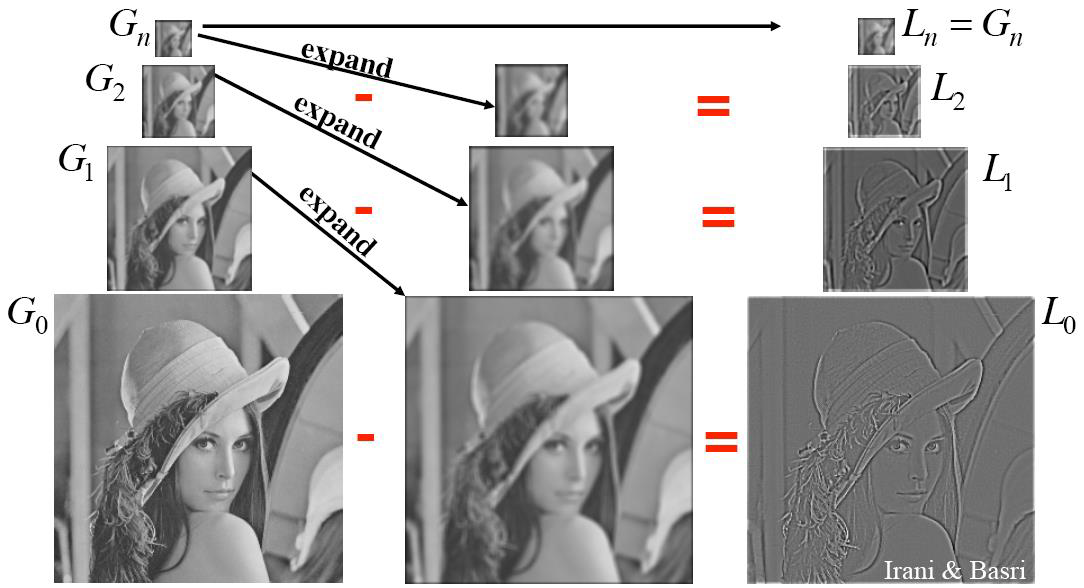
\includegraphics[width=0.7\textwidth]{images/laplacian-pyramid}
    \caption[Laplacian Pyramid]{Laplacian Pyramid}
    \label{fig:laplacian-pyramid}
\end{figure}


\subsection{Hough Transform}\label{sec:bif-hough}

Edges can result from: object-background boundaries, object-object boundaries, shadows, discontinuities of object texture, discontinuities of surface normals.

We are interested in finding objects, thus we should discriminate among those types of edges. An approach is to assemble detected edges to extract object contours, even if they not necessarily correspond to object boundaries. \textbf{Hough Transformation} uses the knowledge that many contours belong to straight lines.

A line is represented as $y = ax + b$:
\begin{myitem}
    \item the parameters $a$ and $b$ determine all the points of a line, which corresponds to a transformation: $(a,b) \longrightarrow (x,y)$, that is $y = ax + b$,
    \item inverse interpretation: transformation of $(x,y) \longrightarrow (a,b)$, that is $b = (-x)a + y$.
\end{myitem}
We can use this to conclude that the points for which the magnitude of the first derivative is large lie potentially on a line.

\textit{Idea}: for a particular point $(x,y)$, determine all lines which go through this point, with parameters given by $b = (-x)a + y$; i.e., those lines are given by a line in the parameter space $(a,b)$.

\textit{Implementation}:
\begin{myitem}
    \item the parameter space $(a,b)$ has to be discretized,
    \item for each candidate $(x,y)$ for a line, store the line $b = (-a) x + y$,
    \item in principle, each candidate $(x,y)$ votes for the discretized parameters,
    \item the maxima in the parameter space $(a,b)$ correspond to lines in the image.
\end{myitem}

But this parameterization has two issues: the parameter $a$ can become infinite for vertical lines, the discretization is problematic. Thus, it is used another parameterization with limited domain: $x \cos(\theta) + y \sin(\theta) = \rho$, where $\rho$ is limited by the size of the image and $\theta \in [0, 2 \pi]$.

\begin{figure}[!h]
    \centering
    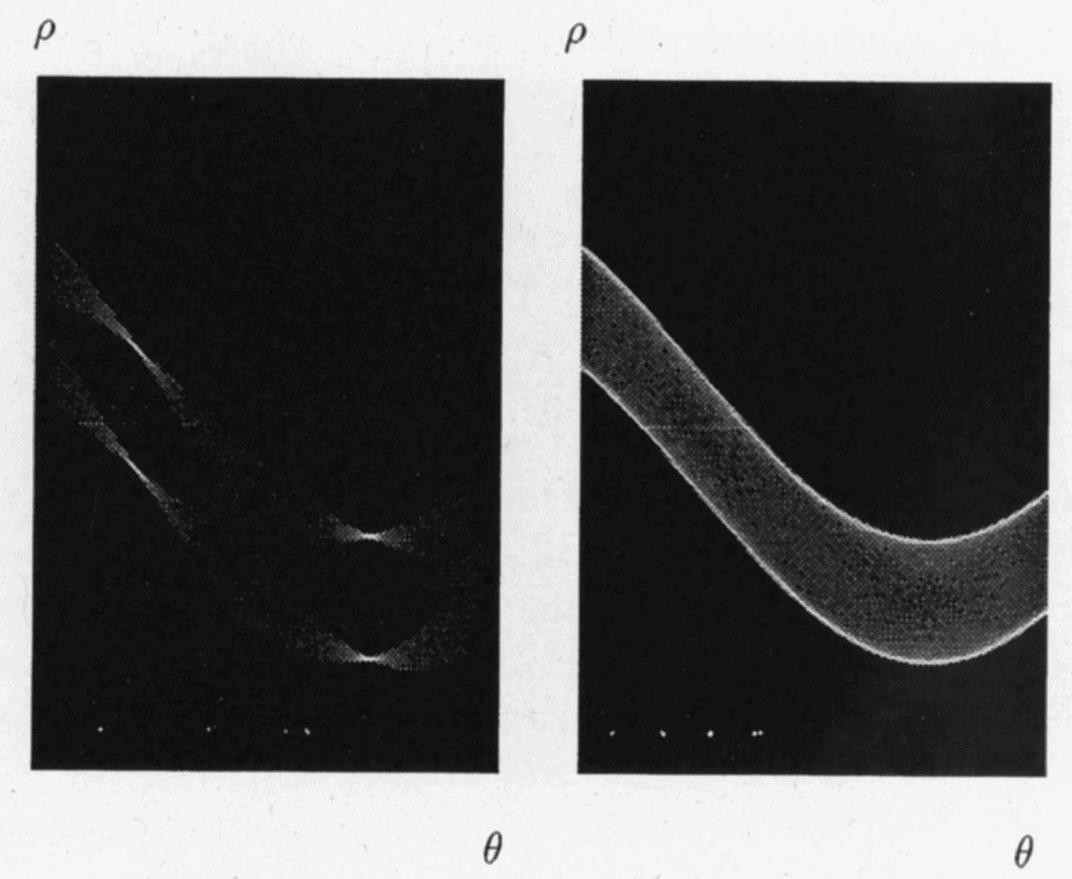
\includegraphics[width=0.7\textwidth]{images/hough-transform}
    \caption[Hough transform]{Hough transform for a square (left) and a circle (right).}
    \label{fig:hough-transform}
\end{figure}

The same idea can be used for other parameterized contours, such as the circle $(x-a)^2 + (y-b)^2 = r^2$, with three parameters: center point $(a, b)$ and radius $r$; but there are some limitations: the parameter space should not become too large and not all contours can be parameterized.

\textbf{Generalization for an arbitrary contour}:
\begin{myitem}
    \item choose reference point for the contour,
    \item for each point on the contour, remember where it is located with respect to the reference point,
    \item recognition: whenever you find a contour point, calculate the tangent angle and \textit{vote} for all possible reference points.
\end{myitem}

